%%% Preamble
\documentclass[paper=letter, fontsize=11pt]{scrartcl}

\usepackage[english]{babel}                                                         % English language/hyphenation
\usepackage[protrusion=true,expansion=true]{microtype}  
\usepackage{amsmath,amsfonts,amsthm} % Math packages
\usepackage[pdftex]{graphicx}   
\usepackage{url}
\usepackage{array}

%%% Custom sectioning
\usepackage{sectsty}
\allsectionsfont{\normalfont\scshape}


%%% Custom headers/footers (fancyhdr package)
\usepackage{fancyhdr}
\pagestyle{fancyplain}
\fancyhead{}                                            % No page header
\fancyfoot[L]{}                                         % Empty 
\fancyfoot[C]{}                                         % Empty
\fancyfoot[R]{\thepage}                                 % Pagenumbering
\renewcommand{\headrulewidth}{0pt}          % Remove header underlines
\renewcommand{\footrulewidth}{0pt}              % Remove footer underlines
\setlength{\headheight}{13.6pt}


%%% Equation and float numbering
\numberwithin{equation}{section}        % Equationnumbering: section.eq#
\numberwithin{figure}{section}          % Figurenumbering: section.fig#
\numberwithin{table}{section}               % Tablenumbering: section.tab#


%%% Maketitle metadata
\newcommand{\horrule}[1]{\rule{\linewidth}{#1}}     % Horizontal rule

\title{
        %\vspace{-1in}  
        \usefont{OT1}{bch}{b}{n}
        \normalfont \normalsize \textsc{TFS Quals Compendium} \\ [25pt]
        \horrule{0.5pt} \\[0.4cm]
        \huge Heat Transfer \\
        \horrule{2pt} \\[0.5cm]
}
\author{
        \normalfont                                 \normalsize
        Andrew Kurzawski\\[-3pt]      \normalsize
        \today
}
\date{}


%%% Begin document
\begin{document}
\maketitle

% \begin{equation}
% \end{equation}

\section{Introduction to Conduction}

Fourier's Law 
\begin{equation}
q_x = -kA\frac{dT}{dx}
\end{equation}

Derive the heat equation in Cartesian, cylindrical, and spherical coordinates. Control volumes defined by the following dimensions: cylindrical $dr, rd\phi, dz$ and spherical $dr, rd\theta, rsin\theta d\phi$.

\bigskip Good Problems: 2.48


\section{1D, Steady-State Conduction}

Thermal Circuits for cartesian and radial systems. Resistances:

\begin{equation}
Cartesian:\quad \frac{L}{kA}
\end{equation}
\begin{equation}
Cylindrical:\quad \frac{ln(r_2/r_1)}{2\pi Lk}
\end{equation}
\begin{equation}
Spherical:\quad \frac{(1/r_1)-(1/r_2)}{4\pi k}
\end{equation}

Integral from of Fourier's Law.

\begin{equation}
q_x\int_{x_o}^x \frac{dx}{A(x)} = -\int_{T_o}^T k(T)dT
\end{equation}

Generation from electric current

\begin{equation}
P = IV = IR^2 = \frac{V^2}{R}
\end{equation}

Fins: use excess temperature ($\theta = T(x) - T_\infty$) and solve the 1-D heat equation. Use Biot number for diameter to justify 1-D and use scaling to justify tip conditions.

\bigskip Good Problems: 3.76, 3.100, 3.112


\section{2D, Steady-State Conduction}

Separation of variables section 4.2. Set $\theta(x,y) = X(x)Y(y)$, where $\theta$ is a non-dimensional temperature that simplifies your boundary conditions. The heat equation now looks like:

\begin{equation}
-\frac{1}{X}\frac{d^2X}{dx^2} = \frac{1}{Y}\frac{d^2Y}{dy^2} = \lambda^2
\end{equation}

\bigskip Good Problems: 4.5


\section{Transient Conduction}

Lumped Capacitance:

\begin{equation}
-hA_s\theta = \rho Vc\frac{dT}{dt}, \theta = T-T_\infty
\end{equation}

\begin{equation}
\theta = \theta_i exp\left(-\frac{hA_s}{\rho Vc}t\right)
\end{equation}

This is valid for Biot number $Bi = \frac{hL_c}{k} < 0.1$.

For systems with radiation, we can estimate a radiation heat transfer coefficient with an average surface temperature.

\begin{equation}
h_r = \epsilon\sigma(T_s + T_{sur})(T_s^2 + T_{sur}^2)
\end{equation}

Semi-infinite solid solution, use the similarity variable $\eta = x/(4\alpha t)^{1/2}$

\bigskip Good Problems: 5.1, 5.2 (sketching and writing differential equations), 5.14, 5.17


\section{Introduction to Convection}
Heat transfer coefficient:

\begin{equation}
q = \bar h A_s(T_s-T_\infty), \quad \bar h = \frac{1}{A_s}\int hdA_s
\end{equation}

For laminar boundary layers

\begin{equation}
\frac{\delta}{\delta_t} \approx Pr^n
\end{equation}

\noindent where $n=1/3$ from the Blasius solution for laminar flow over a flat plate.


\section{External Flow}

For external flow, most correlations take the form

\begin{equation}
\overline{Nu}_L = CRe_L^mPr^n
\end{equation}

The Blasius Solution applies to laminar flow over a flat plate with a constant surface temperature. This solution relies on using the stream function 

\begin{equation}
u = \frac{\partial\Psi}{\partial y}\quad and\quad v = -\frac{\partial\Psi}{\partial x}
\end{equation}

\noindent and the following new variables

\begin{equation}
f(\eta) = \frac{\Psi}{u_\infty\sqrt{\nu x/u_\infty}}\quad and\quad \eta = y\sqrt{u_\infty/\nu x}
\end{equation}

From this solution, it can be shown that the laminar momentum boundary layer thickness is

\begin{equation}
\delta = \frac{5x}{\sqrt{Re_x}}
\end{equation}

\noindent and the local friction coefficient is 

\begin{equation}
C_f = \frac{0.664}{\sqrt{Re_x}}
\end{equation}

\bigskip Good Problems 7.25, 7.26


\section{Internal Flow}

Use the fluids text for information on deriving the velocity profile.

For heat transfer analysis we define the mean fluid temperature as

\begin{equation}
T_m = \frac{\int_{A_c} \rho u c_p T dA_c}{\dot m c_p}
\end{equation}

Then we can use Newtons law of cooling with $T_m$ as follows

\begin{equation}
q_s'' = h(T_s - T_m)
\end{equation}

\begin{figure}[!ht]
\centering
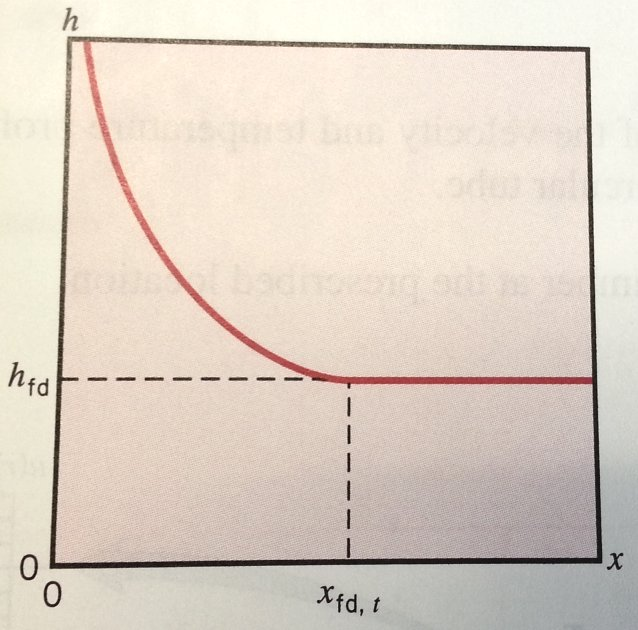
\includegraphics[width=0.5\textwidth]{./Figures/hx}
\caption{Variation of $h(x)$ for developing and fully thermally developed flow.}
\end{figure}

In general, for constant surface heat flux the mean temperature can be expressed as

\begin{equation}
T_m(x) = T_{m,i} + \frac{q_s'' P}{\dot m c_p}x
\end{equation}

\noindent while a constant surface temperature leads to 

\begin{equation}
\frac{T_s - T_m(x)}{T_s - T_{m,i}} = exp\left(-\frac{Px}{\dot m c_p}\bar h\right)
\end{equation}

Both of these equations come from an energy balance on a differential control volume for flow in a tube.

For laminar, fully-developed flow in circular tubes, the Nusselt number is constant. $Nu_D = 4.36$ for constant surface heat flux and $Nu_D=3.66$ for constant surface temperature. You should be able to prove this.

Hydraulic diameter for non-circular ducts

\begin{equation}
D_h = \frac{4A_c}{P}
\end{equation}

\bigskip Good Problems: 8.5, 8.12, 8.53, 8.79


\section{Free Convection}

Natural convection between plates Fig 9.1

Volumetric thermal expansion coefficient 

\begin{equation}
\beta = -\frac{1}{\rho}\left(\frac{\partial\rho}{\partial T}\right)_p
\end{equation}

To get the Grashof Number, we use the scaling variables $x^\ast = \frac{x}{L}$, $y^\ast = \frac{y}{L}$, $u^\ast = \frac{u}{u_0}$, $v^\ast = \frac{v}{u_0}$ and $T^\ast = \frac{T-T_\inft}{T_s-T_\inft}$ to reduce the x-momentum and energy equations.

For external free convection, Nusselt number correlations usually take the form

\begin{equation}
\overline{Nu}_L = C Ra_L^n
\end{equation}

\noindent where the Rayleigh dictates whether the flow is laminar or turbulent, with a critical value of around $10^9$ for vertical flat plates.
    

\section{Heat Exchangers}

Know how to sketch temperature profiles for parallel and counter flow heat exchangers.

Log mean temperature difference 

\begin{equation}
q = UA\Delta T_{lm}
\end{equation}

\noindent where

\begin{equation}
\Delta T_{lm} = \frac{\Delta T_2 - \Delta T_1}{ln(\Delta T_2 / \Delta T_1)}
\end{equation}

\noindent and $\Delta T_i$ is the local temperature difference between the hot and cold streams at point $i$.


\section{Radiation: Processes and Properties}

Solid Angle:

\begin{equation}
d\omega = \frac{dA_n}{r^2}
\end{equation}

Diffuse emitter - a surface for which the intensity of the emitted radiation is independent of direction.

Radiation Intensity:

\begin{equation}
dq_\lambda = I_{\lambda,e}(\lambda,\theta,\phi)dA_1cos\theta d\omega
\end{equation}

Emissive power:

\begin{equation}
E_\lambda(\lambda) = dq_\lambda'' = \frac{dq_\lambda}{dA_1}
\end{equation}

\noindent for a diffuse emitter

\begin{equation}
E_\lambda(\lambda) = \pi I_{\lambda,e}(\lambda)
\end{equation}

Similarly for irradiation where $I_{\lambda,i}$ is the incident spectral intensity from surface $i$. For the diffuse case this is

\begin{equation}
G_\lambda(\lambda) = \pi I_{\lambda,i}(\lambda)
\end{equation}

Radiosity is the reflected and emitted radiation from a surface.

\begin{equation}
J_\lambda(\lambda) = \int_0^{2\pi}\int_0^{\pi/2} I_{\lambda,e+r}(\lambda,\theta,\phi)cos\theta sin\theta d\theta d\phi
\end{equation}

\noindent For the diffuse case this becomes

\begin{equation}
J_\lambda(\lambda) = \pi I_{\lambda,e+r}(\lambda)
\end{equation}

Blackbody - absorbs all incident radiation, regardless of wavelength and direction. For a prescribed temperature and wavelength, no surface can emit more energy than a blackbody. A blackbody is diffuse, but still depends on wavelength and temperature. (The sun can be approximated as a blackbody at 5800 K.)

Wien’s displacement law

\begin{equation}
\lambda_{max}T = 2898 \mu mK
\end{equation}

Stefan-Boltzman Law

\begin{equation}
E_b = \sigma T^4, \quad \sigma = 5.670e-8 \frac{W}{m^2K^4}
\end{equation}

Band Emission

\begin{equation}
F_{(0\rightarrow\lambda)} = \frac{\int_0^\lambda E_{\lambda,b}d\lambda}{\sigma T^4}
\end{equation}

\begin{equation}
F_{(\lambda_1\rightarrow\lambda_2)} = \frac{\int_0^{\lambda_2} E_{\lambda,b}d\lambda - \int_0^{\lambda_1} E_{\lambda,b}d\lambda}{\sigma T^4} = F_{(0\rightarrow\lambda_2)} - F_{(0\rightarrow\lambda_1)}
\end{equation}

\begin{table}[!ht]
\caption{Surface Radiation Properties.}
\centering
  \begin{tabular}{ c | c c c c}
    \noalign{\smallskip}
    Property & Emissivity $\epsilon(T)$ & Absorptivity $\alpha$ & Reflectivity $\rho$ & Transmissivity $\tau$ \\
    \noalign{\smallskip}\hline\noalign{\smallskip}
    Equation  & $ \frac{\int_0^\infty \epsilon_\lambda(\lambda,T)E_{\lambda,b}(\lambda,T)d\lambda}{E_b(T)}$ & $\frac{\int_0^\infty \alpha_\lambda(\lambda)G_{\lambda}(\lambda)d\lambda}{\int_0^\infty G_{\lambda}(\lambda)d\lambda}$ & $\frac{\int_0^\infty \rho_\lambda(\lambda)G_{\lambda}(\lambda)d\lambda}{\int_0^\infty G_{\lambda}(\lambda)d\lambda}$ & $\frac{\int_0^\infty \tau_\lambda(\lambda)G_{\lambda}(\lambda)d\lambda}{\int_0^\infty G_{\lambda}(\lambda)d\lambda}$ \\
  \end{tabular}
\end{table}

Using an irradiation balance for a semi-transparent surface, we get

\begin{equation}
G_\lambda = G_{\lambda,ref} + G_{\lambda,abs} + G_{\lambda,tr}
\end{equation}

\noindent which reduces to

\begin{equation}
1 = \rho_\lambda + \alpha_\lambda + \tau_\lambda
\end{equation}

For an opaque surface where there is no transmission, this reduces to

\begin{equation}
1 = \rho_\lambda + \alpha_\lambda
\end{equation}

Kirchoff’s Law - for small bodies in an isothermal enclosure, at equilibrium all temperatures must be equal and $\alpha=\epsilon$ for any surface in the enclosure.

Gray surface - $\alpha_\lambda$ and $\epsilon_\lambda$ are independent of $\lambda$ over the spectral regions of the irradiation and the surface emission. See Fig 12.26

\bigskip Good Problems: 12.3, 12.26


\section{Radiation Exchange Between Surfaces}

View Factor Integral:

\begin{equation}
F_{ij} = \frac{1}{A_i}\int\int\frac{cos\theta_icos\theta_j}{\pi R^2}dA_idA_j
\end{equation}

Reciprocity and summation rules for view factors:

\begin{equation}
A_i F_{ij} = A_j F_{ji},\quad \sum_{j=1}^N F_{ij} = 1
\end{equation}

Hottel’s cross string rule for 2-D surfaces

\begin{equation}
F_{12} = \frac{\sum crosses-\sum edges}{2A_1}
\end{equation}

Radiation exchange between opaque, diffuse, gray surfaces in an enclosure:

\begin{figure}[!ht]
\centering
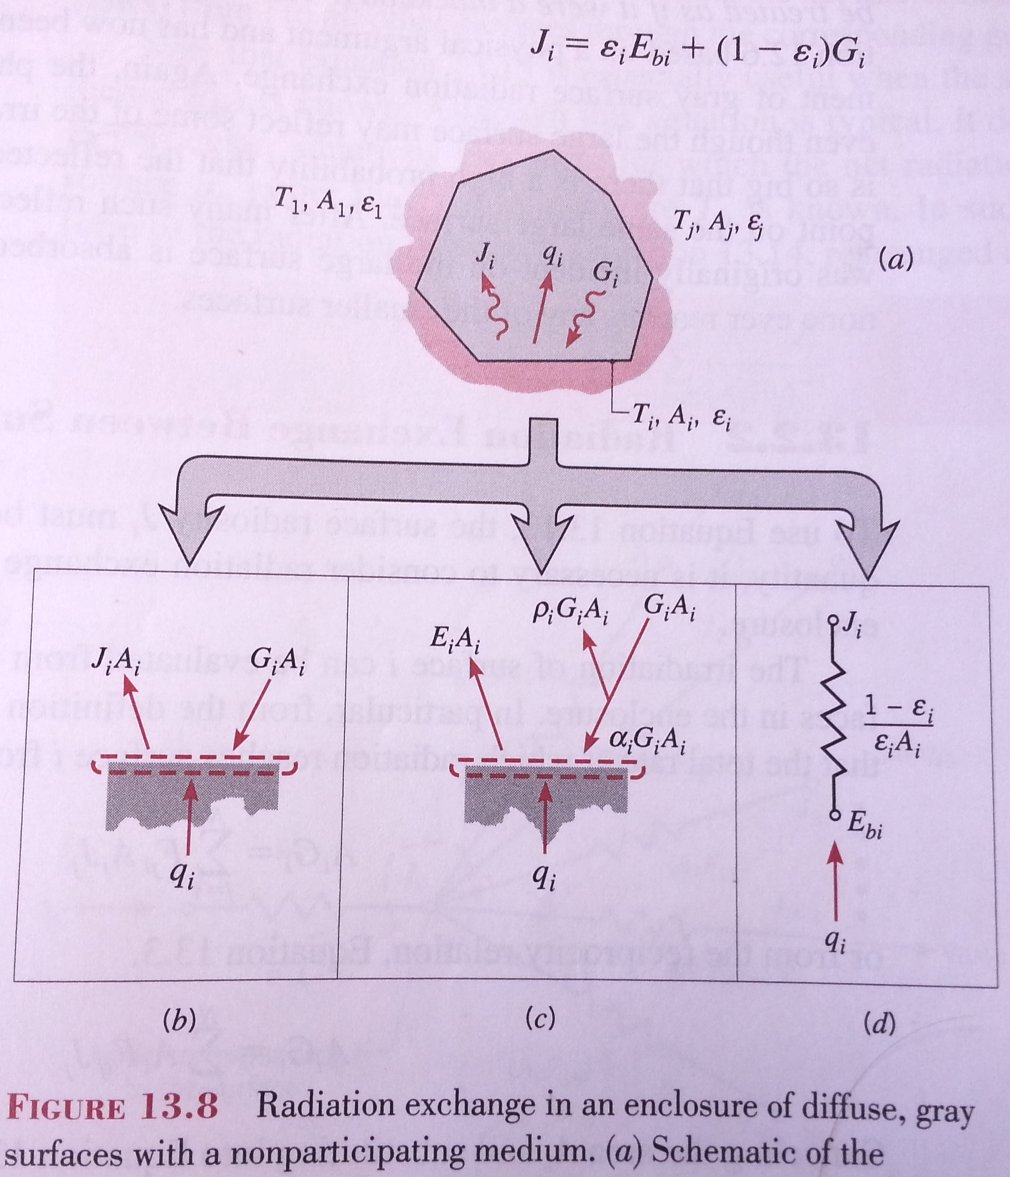
\includegraphics[width=0.6\textwidth]{./Figures/radiation_surface}
\end{figure}

\begin{equation}
q_i = \frac{E_{bi}-J_i}{(1-\epsilon_i)/\epsilon_iA_i}
\end{equation}

\begin{equation}
q_i = \sum_{j=1}^N A_i F_{ij} (J_i-J_j)
\end{equation}

\begin{equation}
\frac{E_{bi}-J_i}{(1-\epsilon_i)/\epsilon_iA_i} = \sum_{j=1}^N A_i F_{ij} (J_i-J_j)
\end{equation}

\begin{figure}[!ht]
\centering
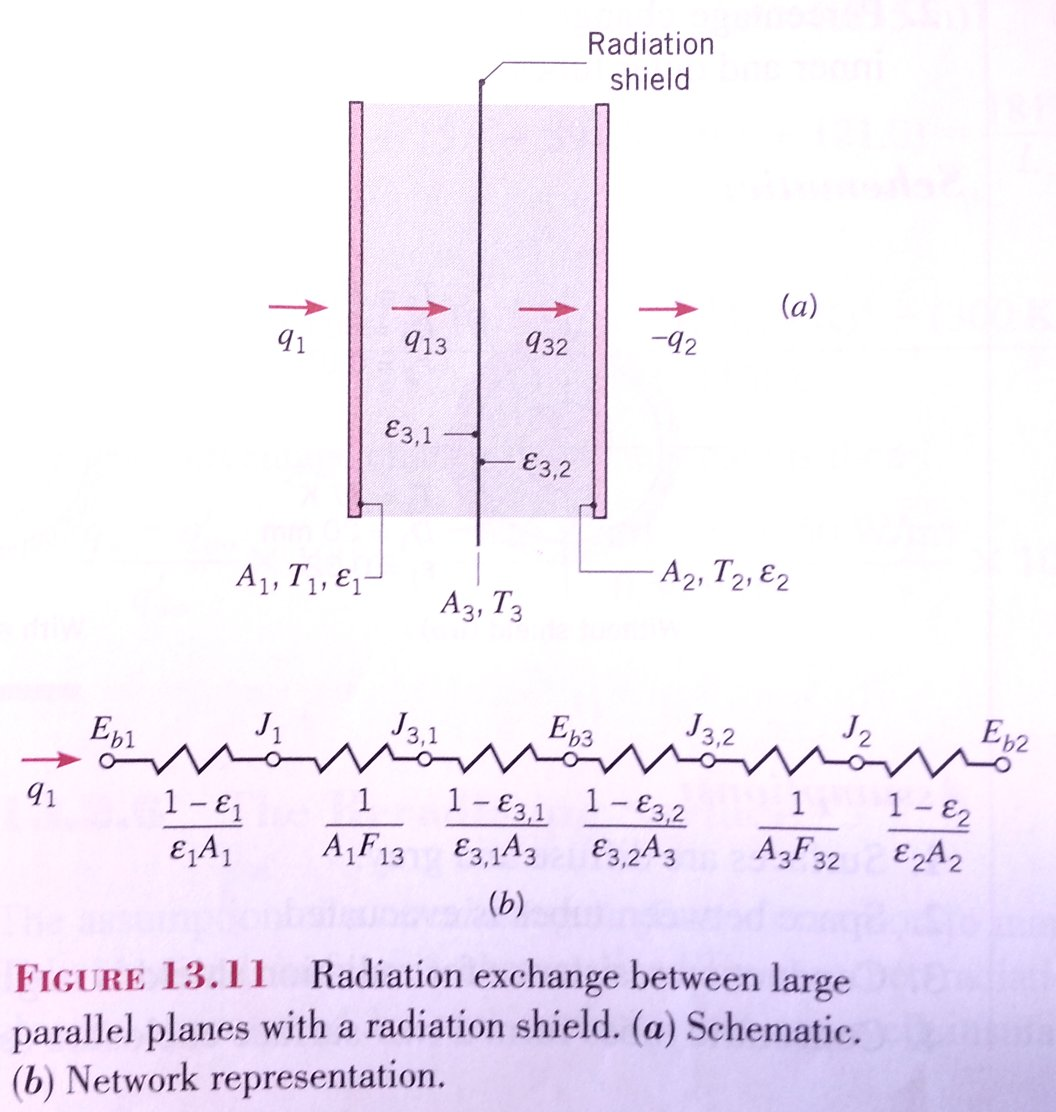
\includegraphics[width=0.6\textwidth]{./Figures/radiation_shield}
\end{figure}

\begin{figure}[!ht]
\centering
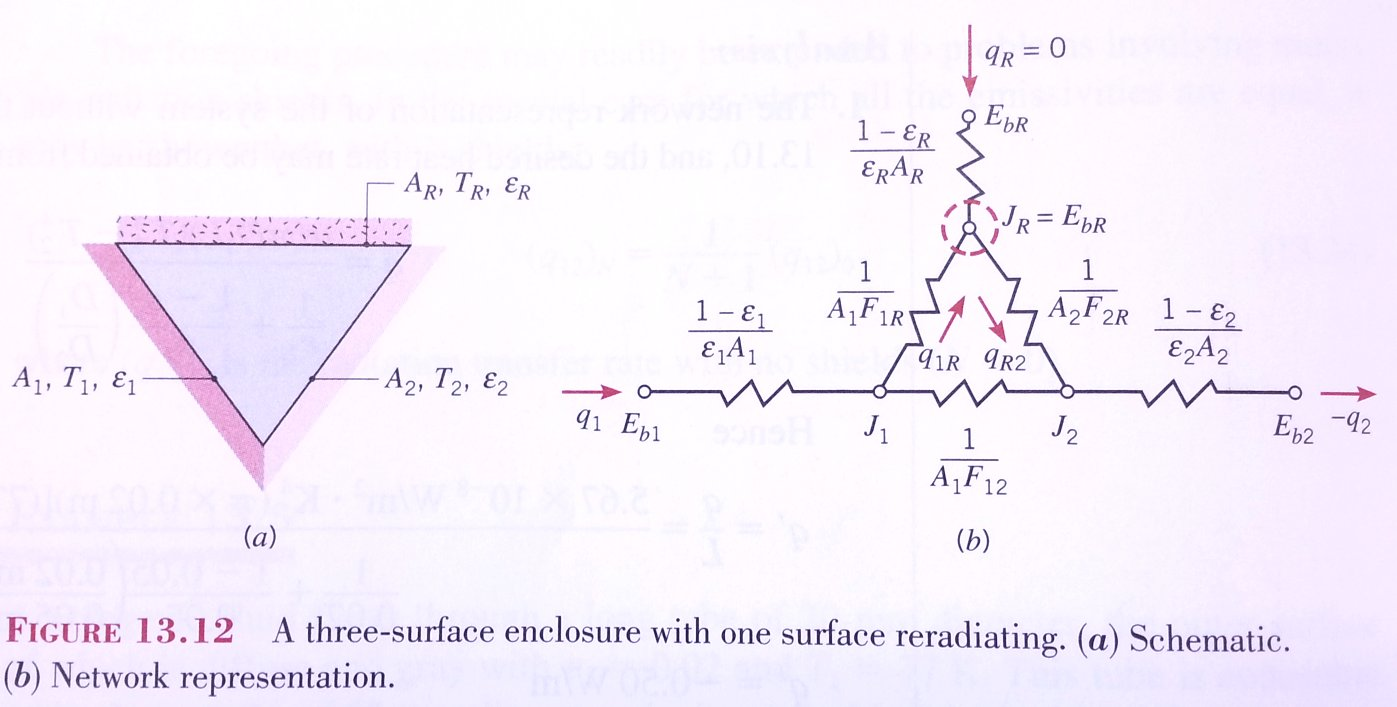
\includegraphics[width=0.9\textwidth]{./Figures/three_surface}
\end{figure}

\bigskip Good Problems: 13.63, 13.100

\clearpage
\section{Dimensionless Numbers}

\begin{table}[!ht]
\caption{Useful Dimensionless Numbers.}
\centering
  \begin{tabular}{ c c m{8cm}}
    \noalign{\smallskip}
    Name & Definition & Interpretation \\
    \noalign{\smallskip}\hline\noalign{\smallskip}
    $Bi$  & $\frac{hL}{k}$ & Ratio of the internal thermal resistance of a solid to the boundary layer thermal resistance \\
    $C_f$ & $\frac{\tau_s}{\rho V^2/2}$ & Dimensionless surface shear stress \\
    $Fo$  & $\frac{\alpha t}{L^2}$ & Ratio of the heat conduction rate to the rate of thermal energy storage in a solid \\
    $f$   & $\frac{\Delta p}{(L/D)(\rho u_m^2/2)}$ & Dimensionless pressure drop for internal flow \\
    $Gr$  & $\frac{g\beta(T_s-T_\infty)L^3}{\nu^2}$ & Measure of the ratio of buoyancy forces to viscous forces \\
    $Nu$  & $\frac{hL}{k_f}$ & Ratio of convection to pure conduction heat transfer \\
    $Pe$  & $\frac{VL}{\alpha}=Re_LPr$ & Ratio of advection to conduction heat transfer rates \\
    $Pr$  & $\frac{\nu}{\alpha}$ & Ratio of momentum to thermal diffusion \\
    $Ra$  & $\frac{g\beta(T_s-T_\infty)L^3}{\nu\alpha}$ & $GrPr$ \\
    $Re$  & $\frac{\rho V L}{\mu}$ & Ratio of inertia and viscous forces \\
    \noalign{\smallskip}\hline
  \end{tabular}
\end{table}

%%% End document
\end{document}
